\documentclass[twoside]{book}

% Packages required by doxygen
\usepackage{fixltx2e}
\usepackage{calc}
\usepackage{doxygen}
\usepackage[export]{adjustbox} % also loads graphicx
\usepackage{graphicx}
\usepackage[utf8]{inputenc}
\usepackage{makeidx}
\usepackage{multicol}
\usepackage{multirow}
\PassOptionsToPackage{warn}{textcomp}
\usepackage{textcomp}
\usepackage[nointegrals]{wasysym}
\usepackage[table]{xcolor}

% Font selection
\usepackage[T1]{fontenc}
\usepackage[scaled=.90]{helvet}
\usepackage{courier}
\usepackage{amssymb}
\usepackage{sectsty}
\renewcommand{\familydefault}{\sfdefault}
\allsectionsfont{%
  \fontseries{bc}\selectfont%
  \color{darkgray}%
}
\renewcommand{\DoxyLabelFont}{%
  \fontseries{bc}\selectfont%
  \color{darkgray}%
}
\newcommand{\+}{\discretionary{\mbox{\scriptsize$\hookleftarrow$}}{}{}}

% Page & text layout
\usepackage{geometry}
\geometry{%
  a4paper,%
  top=2.5cm,%
  bottom=2.5cm,%
  left=2.5cm,%
  right=2.5cm%
}
\tolerance=750
\hfuzz=15pt
\hbadness=750
\setlength{\emergencystretch}{15pt}
\setlength{\parindent}{0cm}
\setlength{\parskip}{3ex plus 2ex minus 2ex}
\makeatletter
\renewcommand{\paragraph}{%
  \@startsection{paragraph}{4}{0ex}{-1.0ex}{1.0ex}{%
    \normalfont\normalsize\bfseries\SS@parafont%
  }%
}
\renewcommand{\subparagraph}{%
  \@startsection{subparagraph}{5}{0ex}{-1.0ex}{1.0ex}{%
    \normalfont\normalsize\bfseries\SS@subparafont%
  }%
}
\makeatother

% Headers & footers
\usepackage{fancyhdr}
\pagestyle{fancyplain}
\fancyhead[LE]{\fancyplain{}{\bfseries\thepage}}
\fancyhead[CE]{\fancyplain{}{}}
\fancyhead[RE]{\fancyplain{}{\bfseries\leftmark}}
\fancyhead[LO]{\fancyplain{}{\bfseries\rightmark}}
\fancyhead[CO]{\fancyplain{}{}}
\fancyhead[RO]{\fancyplain{}{\bfseries\thepage}}
\fancyfoot[LE]{\fancyplain{}{}}
\fancyfoot[CE]{\fancyplain{}{}}
\fancyfoot[RE]{\fancyplain{}{\bfseries\scriptsize Generated by Doxygen }}
\fancyfoot[LO]{\fancyplain{}{\bfseries\scriptsize Generated by Doxygen }}
\fancyfoot[CO]{\fancyplain{}{}}
\fancyfoot[RO]{\fancyplain{}{}}
\renewcommand{\footrulewidth}{0.4pt}
\renewcommand{\chaptermark}[1]{%
  \markboth{#1}{}%
}
\renewcommand{\sectionmark}[1]{%
  \markright{\thesection\ #1}%
}

% Indices & bibliography
\usepackage{natbib}
\usepackage[titles]{tocloft}
\setcounter{tocdepth}{3}
\setcounter{secnumdepth}{5}
\makeindex

% Hyperlinks (required, but should be loaded last)
\usepackage{ifpdf}
\ifpdf
  \usepackage[pdftex,pagebackref=true]{hyperref}
\else
  \usepackage[ps2pdf,pagebackref=true]{hyperref}
\fi
\hypersetup{%
  colorlinks=true,%
  linkcolor=blue,%
  citecolor=blue,%
  unicode%
}

% Custom commands
\newcommand{\clearemptydoublepage}{%
  \newpage{\pagestyle{empty}\cleardoublepage}%
}

\usepackage{caption}
\captionsetup{labelsep=space,justification=centering,font={bf},singlelinecheck=off,skip=4pt,position=top}

%===== C O N T E N T S =====

\begin{document}

% Titlepage & ToC
\hypersetup{pageanchor=false,
             bookmarksnumbered=true,
             pdfencoding=unicode
            }
\pagenumbering{roman}
\begin{titlepage}
\vspace*{7cm}
\begin{center}%
{\Large My Project }\\
\vspace*{1cm}
{\large Generated by Doxygen 1.8.11}\\
\end{center}
\end{titlepage}
\clearemptydoublepage
\tableofcontents
\clearemptydoublepage
\pagenumbering{arabic}
\hypersetup{pageanchor=true}

%--- Begin generated contents ---
\chapter{Hierarchical Index}
\section{Class Hierarchy}
This inheritance list is sorted roughly, but not completely, alphabetically\+:\begin{DoxyCompactList}
\item \contentsline{section}{Class\+\_\+\+Jetson\+\_\+\+Buttons}{\pageref{classClass__Jetson__Buttons}}{}
\item Q\+Main\+Window\begin{DoxyCompactList}
\item \contentsline{section}{Main\+Window}{\pageref{classMainWindow}}{}
\end{DoxyCompactList}
\end{DoxyCompactList}

\chapter{Class Index}
\section{Class List}
Here are the classes, structs, unions and interfaces with brief descriptions\+:\begin{DoxyCompactList}
\item\contentsline{section}{\hyperlink{classClass__Jetson__Buttons}{Class\+\_\+\+Jetson\+\_\+\+Buttons} }{\pageref{classClass__Jetson__Buttons}}{}
\item\contentsline{section}{\hyperlink{classMainWindow}{Main\+Window} }{\pageref{classMainWindow}}{}
\end{DoxyCompactList}

\chapter{Class Documentation}
\hypertarget{classClass__Jetson__Buttons}{}\section{Class\+\_\+\+Jetson\+\_\+\+Buttons Class Reference}
\label{classClass__Jetson__Buttons}\index{Class\+\_\+\+Jetson\+\_\+\+Buttons@{Class\+\_\+\+Jetson\+\_\+\+Buttons}}
\subsection*{Public Member Functions}
\begin{DoxyCompactItemize}
\item 
\hyperlink{classClass__Jetson__Buttons_ad738a87617369bfeda09a07fceec25cb}{Class\+\_\+\+Jetson\+\_\+\+Buttons} ()\hypertarget{classClass__Jetson__Buttons_ad738a87617369bfeda09a07fceec25cb}{}\label{classClass__Jetson__Buttons_ad738a87617369bfeda09a07fceec25cb}

\begin{DoxyCompactList}\small\item\em Construct a new \hyperlink{classClass__Jetson__Buttons_ad738a87617369bfeda09a07fceec25cb}{Class\+\_\+\+Jetson\+\_\+\+Buttons\+::\+Class\+\_\+\+Jetson\+\_\+\+Buttons} object. \end{DoxyCompactList}\item 
void \hyperlink{classClass__Jetson__Buttons_ac93e60e7ed8d1e861f2f571151407d7d}{Button\+Out\+Put} (out int pin\+Name, out int Status)
\begin{DoxyCompactList}\small\item\em Construct a new \hyperlink{classClass__Jetson__Buttons_ac93e60e7ed8d1e861f2f571151407d7d}{Class\+\_\+\+Jetson\+\_\+\+Buttons\+::\+Button\+Out\+Put} object. \end{DoxyCompactList}\end{DoxyCompactItemize}


\subsection{Member Function Documentation}
\index{Class\+\_\+\+Jetson\+\_\+\+Buttons@{Class\+\_\+\+Jetson\+\_\+\+Buttons}!Button\+Out\+Put@{Button\+Out\+Put}}
\index{Button\+Out\+Put@{Button\+Out\+Put}!Class\+\_\+\+Jetson\+\_\+\+Buttons@{Class\+\_\+\+Jetson\+\_\+\+Buttons}}
\subsubsection[{\texorpdfstring{Button\+Out\+Put(out int pin\+Name, out int Status)}{ButtonOutPut(out int pinName, out int Status)}}]{\setlength{\rightskip}{0pt plus 5cm}Class\+\_\+\+Jetson\+\_\+\+Buttons\+::\+Button\+Out\+Put (
\begin{DoxyParamCaption}
\item[{out int}]{pin\+Name, }
\item[{out int}]{Status}
\end{DoxyParamCaption}
)}\hypertarget{classClass__Jetson__Buttons_ac93e60e7ed8d1e861f2f571151407d7d}{}\label{classClass__Jetson__Buttons_ac93e60e7ed8d1e861f2f571151407d7d}


Construct a new \hyperlink{classClass__Jetson__Buttons_ac93e60e7ed8d1e861f2f571151407d7d}{Class\+\_\+\+Jetson\+\_\+\+Buttons\+::\+Button\+Out\+Put} object. 


\begin{DoxyParams}{Parameters}
{\em int} & pin\+Name\+: Pin name in hardware \\
\hline
{\em int} & Status\+: high or low \\
\hline
\end{DoxyParams}


The documentation for this class was generated from the following files\+:\begin{DoxyCompactItemize}
\item 
class\+\_\+jetson\+\_\+buttons.\+h\item 
class\+\_\+jetson\+\_\+buttons.\+cpp\end{DoxyCompactItemize}

\hypertarget{classMainWindow}{}\section{Main\+Window Class Reference}
\label{classMainWindow}\index{Main\+Window@{Main\+Window}}


Inheritance diagram for Main\+Window\+:\nopagebreak
\begin{figure}[H]
\begin{center}
\leavevmode
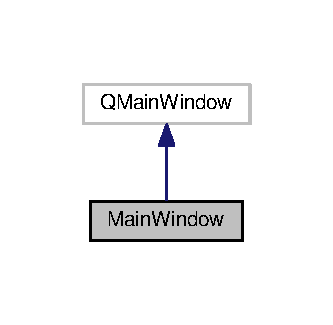
\includegraphics[width=160pt]{classMainWindow__inherit__graph}
\end{center}
\end{figure}


Collaboration diagram for Main\+Window\+:\nopagebreak
\begin{figure}[H]
\begin{center}
\leavevmode
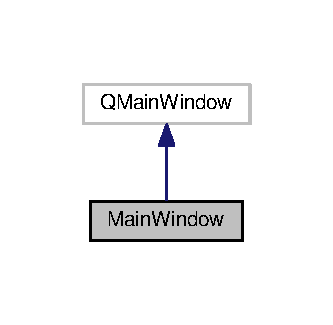
\includegraphics[width=160pt]{classMainWindow__coll__graph}
\end{center}
\end{figure}
\subsection*{Public Member Functions}
\begin{DoxyCompactItemize}
\item 
{\bfseries Main\+Window} (Q\+Widget $\ast$parent=0)\hypertarget{classMainWindow_a8b244be8b7b7db1b08de2a2acb9409db}{}\label{classMainWindow_a8b244be8b7b7db1b08de2a2acb9409db}

\end{DoxyCompactItemize}


The documentation for this class was generated from the following files\+:\begin{DoxyCompactItemize}
\item 
mainwindow.\+h\item 
mainwindow.\+cpp\end{DoxyCompactItemize}

%--- End generated contents ---

% Index
\backmatter
\newpage
\phantomsection
\clearemptydoublepage
\addcontentsline{toc}{chapter}{Index}
\printindex

\end{document}
